\section{Methods}

\subsection{Multimeter connection}
It posed a challenge to establish the Computer-Arduino-Multimeter communication. Originally, the goal was to use the oscilloscope RIGOL MSO1104 Z but we couldn't find the drive needed to connect it to the computer. Eventually, we ended up using the multimeter Agilent 34401A 61/2 Digit Multimeter\cite{keysight34401A}. 

The most prominent difficulty was that the multimeter received commands but did not transmit anything back. For example, when sending a MEAS:VOLT:DC? command, the voltage was displayed on the multimeter screen but not sent to the computer. This was resolved after adjusting the MAX3232 connector. A 3.5kOhm pull-up resistor was utilized and connected as shown in \ref{MAX3232}.

\begin{figure}[H]
          \centering
          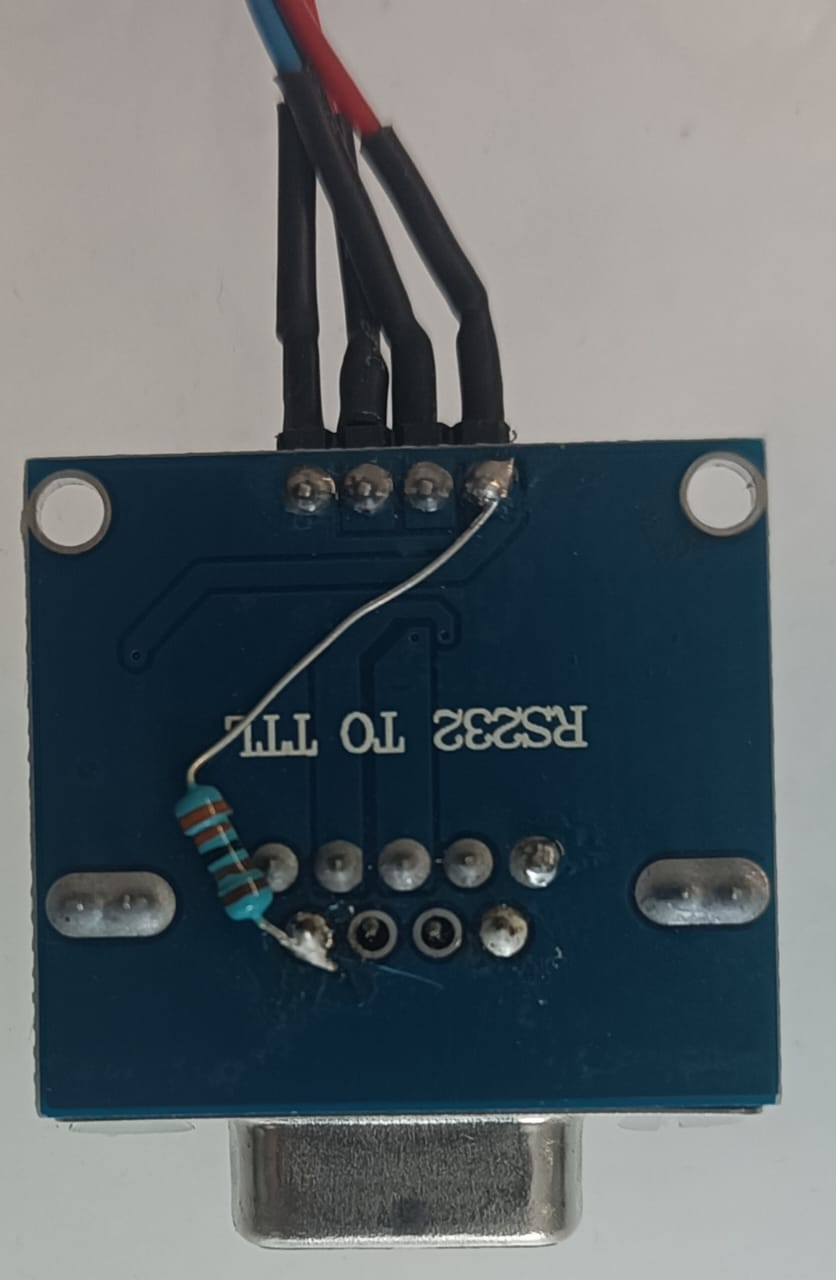
\includegraphics[angle=90, width=0.5\textwidth]{img/RS232_connector.jpeg}
          \caption{Picture of MAX3232 with 3.5kOhm pull-up resistor.}
          \label{MAX3232}
    \end{figure}

Some code that successfully enables communication between an Arduino DUE and the multimeter can be found in the project under Code that worked. This is useful to test initial communication with the multimeter. The connections of the Arduino DUE and the MAX3232 module are as shown in Figure \ref{MAX3232_Arduino}.

\begin{figure}[H]
          \centering
          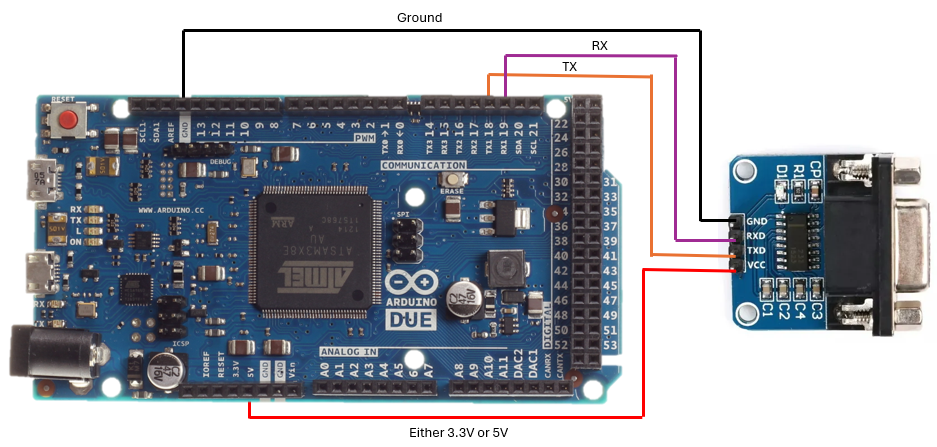
\includegraphics[width=1\linewidth]{img/MAX3232_connection.png}
          \caption{Electrical connection of Arduino DUE and MAX3232.}
          \label{MAX3232_Arduino}
    \end{figure}


\subsection{PCB version 1}
After some prototyping with a breadboard, the first version of the PCB was developed. It was given the name 'Automated DMM tester V1'. The purpose of this version is to test everything works smoothly and identify areas of improvement. 

A 16 channel MUX was chosen to direct the current of each ePATH pin to the multimeter so that the tests can be performed. A MUX was chosen over alternatives, such as shift registers with relays, for its simple wiring and fast operation \cite{tiMAX3232guide}. A 16 channeled one was chosen as there are 12 pins to be tested.

The kiCAD design of the PCB is stored in the project as PCB attempt 1. When soldering the components on the board some alternations were made; instead of $330\,\Omega$ resistors, $1.6k\,\Omega$ resistors were used and instead of $10k\,\Omega$ resistors $4.6k\,\Omega$ resistors were used. The Arduino program used on it to test the functionality of the board is saved in the project as PCB programming. 

In the schematic, the $330\,\Omega$ resistors were chosen since the forward voltage drop for white LEDs is approximately 2.4V and the desired current flow through them is about 10mA. Therefore:
\[
R = \frac{V}{I} = \frac{5\,\mathrm{V} - 2.4\,\mathrm{V}}{10\,\mathrm{mA}}=260\Omega
\]
Since $330\,\Omega$ is very close to the desired resistance and is a more readily available resistor value it was chosen.


There was a number of errors with this design:
\begin{itemize}
\item The symbol used for the banana socket is wrong. It represents the banana socket as a one-pin connector but it has 4 connecting terminals. This led to receiving an inquiry about it from the manufacturers.
\item The orientation of the button footprint is incorrect-it should be rotated by 90 degrees. This issue was bypassed when making the button connection to the board but an awkward connection was produced.
\item The wiring of the Restart button is incorrect. It was not connected to the Arduino DUE pin 8 properly. This was corrected on the board according to the diagram in Figure \ref{button_wiring}.
\end{itemize}

\begin{figure}[H]
          \centering
          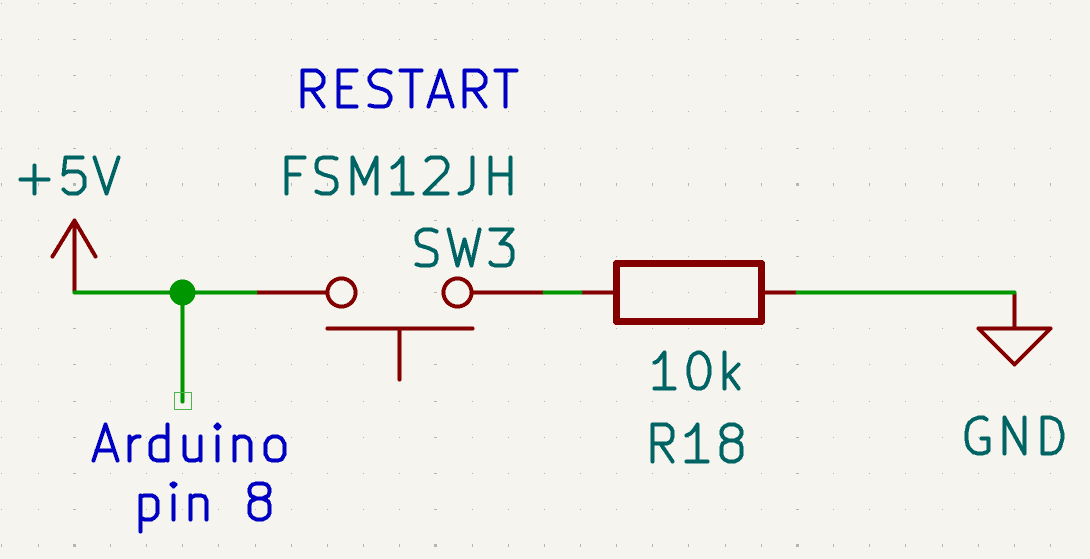
\includegraphics[width=1\linewidth]{img/button_wiring.png}
          \caption{Corrected electrical connection of RESTART button}
          \label{button_wiring}
    \end{figure}



\subsection{PCB version 2}
The improvements made for the second version of the PCB include:
\begin{itemize}
\item Some different electrical components were chosen, such as the MUX, that were more appropriate for the last scale production of the custom PCB board.
\item Implemented a module capable of obtaining the RFID tag of the ePATH board.
\item c
\end{itemize}




\subsection{GUI}
A user friendly GUI has been developed to facilitate the testing of the ePATH PCB. The code for the GUI is on the ePATH-Test-Bench project of the company's GitHub \href{https://github.com/pathfinder-medical/ePATH-Test-Bench}{here}.

The key functionalities of the GUI include:
\begin{itemize}
\item Run button; Starts the testing cycle.
\item Clear button; Deletes all testing results for re-tests.
\item Save button; Saves a pdf file with the table of results.
\item Get button; Gets the RFID of the ePATH board.
\end{itemize}
